%\documentclass[12pt,preprint]{aastex}
\documentclass{emulateapj}
% for \sout
\usepackage{ulem}
% makes sure \em{} is italic rather than underlined (corrects ulem from line above)
\normalem

% for the red MarginPars
\usepackage{color}

% some extra math symbols
\usepackage{mathtools}

% allows Greek symbols to be bold
\usepackage{bm}

% allows comment sections
\usepackage{verbatim}

\newcommand{\rhocutoff}{\rho_\mathrm{cutoff}}
\newcommand{\rhoanelastic}{\rho_\mathrm{anelastic}}

\newcommand{\gcc}{\mathrm{g~cm^{-3} }}
\newcommand{\Tcutoff}{T_\mathrm{cutoff}}

% MarginPars
\setlength{\marginparwidth}{0.75in}
\newcommand{\MarginPar}[1]{\marginpar{\vskip-\baselineskip\raggedright\tiny\sffamily\hrule\smallskip{\color{red}#1}\par\smallskip\hrule}}


\newcommand{\evm}{{(-)}}
\newcommand{\evz}{{(\circ)}}
\newcommand{\evp}{{(+)}}
\newcommand{\enu}{{(\nu)}}



\newcommand{\msolar}{\mathrm{M}_\odot}

\begin{document}

%==========================================================================
% Title
%==========================================================================
\title{Double White Dwarf Mergers with CASTRO\\ I. Methodology and Code 
       Verification}

\shorttitle{DWD Mergers. I. Methodology}
\shortauthors{Katz et al. (2015)}

\author{Max P. Katz, Michael Zingale, Alan C. Calder, F. Douglas Swesty, Ann S. Almgren, Weiqun Zhang}
%==========================================================================
% Abstract
%==========================================================================
\begin{abstract}
The Type Ia supernova progenitor problem is one of the most perplexing and 
exciting problems in astrophysics, requiring detailed numerical modelling to 
complement the observations of these explosions. One possibility that has 
merited recent theoretical attention is the white dwarf merger scenario.
This can naturally explain many of the observed characteristics of 
Type Ia supernovae, as well as their distribution in time and space.
However, to date there have been few fully self-consistent simulations 
of binary white dwarf systems using mesh-based hydrodynamics, 
relative to other methods. This is the first paper in a series designed to 
describe simulations of these systems with the adaptive-mesh refinement 
hydrodynamics code CASTRO. In this paper we describe our numerical 
methodology. CASTRO solves the Euler equations of hydrodynamics 
and the Poisson equation for self-gravity. Standard techniques for 
coupling gravitation and rotation forces to the hydrodynamics do 
not do an adequate job conserving the total energy of the system, 
but recent advances in the literature have made advances on this 
problem and we discuss our implementation here. We also run an 
extensive set of test problems to verify that our software can sufficiently
model a system where large amounts of mass are advected on the computational 
domain over very long timescales. Future papers in this series will describe
our treatment of the initial conditions of these systems, and will 
examine the early phases of the merger to determine its viability
for triggering a thermonuclear detonation.

\end{abstract}
\keywords{hydrodynamics - methods: numerical - supernovae: general - white dwarfs}

%==========================================================================
% Introduction
%==========================================================================
\section{Introduction}

Type Ia supernovae (SNe Ia) are currently some of the most exciting
events to study in astrophysics. These bright, brief pulses of light
in the distant universe have led to a number of important discoveries
in recent years, including the discovery of the accelerated expansion
of the universe \citep{perlmutter1999,riess1998}. However, their
origin is shrouded in mystery. It has long been expected that these
events arise from the thermonuclear explosions of white dwarfs
\citep{hoyle_fowler:1960}, but the cause of these explosions is
uncertain. In particular, it is not clear what process causes the
temperatures in these white dwarfs to become hot enough for explosive
burning of its constituent nuclei. The model favored initially by the
community was the so-called single-degenerate (SD) model
\citep{whelan_iben:1973}. Accretion of material from a companion star
such as a red giant would cause the star to approach the Chandrasekhar
mass, and in doing so the temperature and density in the center would
become sufficient for thermonuclear fusion to proceed. However, in
recent years many alternative progenitor models have been discussed. A
leading candidate for explaining some or most of these explosions is
the double-degenerate (DD) model, in which two white dwarfs merge and
the merged object reaches the conditions necessary for a thermonuclear
ignition \citep{ibentutukov:1984,webbink:1984}. Another is the double
detonation scenario, where accretion of material onto a
sub-Chandrasekhar white dwarf would lead to a detonation inside the
accreted envelope, and this would send a compressional wave into the
core of the star that would trigger a secondary detonation. A recent
review of the progenitor models can be found in
\citet{hillebrandt:2013}.

There are several observational reasons why double-degenerate systems
are a promising progenitor system for at least a substantial fraction
of normal SNe Ia. No conclusive evidence exists for a surviving
companion star of a SN Ia; this is naturally explained by the DD model
because both WDs are likely to be destroyed in the merger
process. Similarly, pre-explosion images of the SN Ia systems have
never clearly turned up a companion star, and in some cases a large
fraction of the parameter space for the nature of the companion star
is excluded. Additionally, not enough progenitor systems are seen for
the SD case to match the observed local SN Ia rate, whereas the number
of white dwarf binaries may be sufficient to account for this
rate. Finally, the DD model can naturally explain the fact that many
SNe Ia are observed to occur at very long delay times after the stars
were formed, since the progenitor systems only become active once both
stars have evolved off the main sequence. A thorough review of the
observational evidence about SNe Ia and further discussion of these
ideas can be found in \cite{maoz:2014}.

The history of double degenerate theory can broadly be described as a
series of three major paradigm shifts. The first attempts to model the
results of the merger process came in the
1980s. \cite{nomotoiben:1985} demonstrated that off-center carbon
ignition would occur in the more massive white dwarf as it accreted
mass near the Eddington rate from the less massive white dwarf
overflowing its Roche lobe. \cite{saionomoto:1985} tracked the
evolution of the flame and found that it propagated quiescently into
the center, converting the carbon-oxygen white dwarf into an
oxygen-neon-magnesium white dwarf. This would then be followed by
collapse into a neutron star -- a result with significantly different
observational properties compared to a SN Ia. This scenario, termed
accretion-induced collapse, would be avoided only if the accretion
rate were well below the Eddington rate. \cite{tutukov_yungelson:1979}
observed that this could happen if the mass loss from the secondary
was higher than the Eddington rate and thus the accreted material
formed an accretion disc, which might rain down on the primary more
slowly. The main finding was that double degenerate systems would not
obviously lead to Type Ia supernovae.

The first three-dimensional simulations of double degenerate systems
were performed by \citet{benz:1990}, who used the smoothed particle
hydrodynamics (SPH) method to simulate the merger process. They found
that if the lower-mass star (generally called the ``secondary'') was
close enough to the more massive star (the ``primary'') to begin mass
transfer on a dynamical time scale, the secondary completely disrupted
and formed a hot envelope around the primary, with a
centrifugally-supported accretion disk surrounding the core and
envelope. They noted that the envelope temperature was hot enough to
generate carbon fusion but neglected nuclear reactions in their
simulation. Later simulations of similar setups
\citep{rasio_shapiro:1995,yoon:2007,loren-aguilar:2009,raskin:2012}
corroborated this result. This validation of the prediction of
\cite{tutukov_yungelson:1979} did not instill confidence in the
community. \cite{mochkovitch_livio:1990} and \cite{livio:2000}
observed that turbulent viscosity would be sufficiently large for
angular momentum to be removed from the disk at a rate high enough to
generate the troublesome accretion timescales. Based on all of this
evidence, the review of \cite{hillebrandtniemeyer2000} argued that the
model was only viable if the accretion-induced collapse problem could
be avoided. Later work by \cite{shen:2012} and \cite{schwab:2012} used
a more detailed treatment of the viscous transport in the outer
regions of the remnant and found that while the centrifugally
supported envelope would be converted into hot envelope material on a
viscous timescale, their simulations still led to off-center carbon
burning. \cite{vankerkwijk:2010} argued that equal-mass mergers would
lead to the conditions necessary for carbon detonation in the center
of the merged object, but \cite{shen:2012} questioned this for similar
reasons related to how viscous transport would convert rotational
motion into pressure support. \cite{zhu:2013} followed this with an
expanded parameter space study and argued that many of their
carbon-oxygen systems had the potential to detonate. The study of the
long-term evolution of the remnants is thus still an open subject of
research.

The most recent shift in perspective on this problem started with two
series of papers appearing at roughly the same time. One began with
\cite{pakmor:2010} and \cite{pakmor:2011}. This group used the SPH
method to study the merger of equal-mass ($0.9\ M_\odot$)
carbon-oxygen white dwarfs and found that a hotspot was generated near
the surface of the primary white dwarf. They argued that this region
had a temperature and density sufficient to trigger a thermonuclear
detonation. They propagated this detonation throughout the system and
found that it would observationally appear as a subluminous Type Ia
supernova. This was the first time a DD simulation successfully
reproduced at least some characteristics of a SN
Ia. \cite{pakmor:2011} tried a few different mass combinations and
found empirically that this would hold as long as the secondary was at
least 80\% as massive as the primary. These events, where the merger
process resulted in the detonation of the system during the merger
coalescence -- avoiding the much longer time-scale evolution -- were
termed ``violent'' mergers.

Around the same time, however, \cite{guillochon:2010} and
\cite{dan:2011} came to significantly different conclusions. They
pointed out that the previously mentioned simulations generally all
shared a significant drawback, which was that their initial conditions
were not carefully constructed. \cite{motl:2002}, \cite{dsouza:2006},
and \cite{motl:2007} (the first three-dimensional grid-based
simulations of mass transfer in binary white dwarf systems) pioneered
the study of looking at the long-term dynamical evolution of binary
white dwarf systems after constructing exact equilibrium initial
conditions. In contrast to the other studies, they found that paying
close attention to the accuracy of the initial conditions of the
simulation has important effects. In particular, earlier work placed
the stars too close together and ignored the effects of tidal forces
on changing the shape of the secondary, leading to the merger
happening artificially too quickly. When the initial conditions are
constructed in exact equilibrium, the system can be stable for tens of
orbital periods, substantially changing the character of the mass
transfer phase. However, one limitation of this series of studies is
that the authors used a polytropic equation of state and thus could
not consider nuclear reactions. \cite{guillochon:2010} and
\cite{dan:2011} improved on this using a realistic equation of state,
a nuclear reaction network, and a similar approach to the equilibrium
initial conditions, and found substantial agreement with the idea that
mass transfer occurs in a stable manner over tens of orbital
periods. They also found that, assuming the material accreted onto the
surface of the primary was primarily helium, explosive surface
detonations would occur as a result of accretion stream instabilities
during the mass transfer phase prior to the full merger. This could
trigger a double-detonation explosion and thus perhaps a SN Ia.

The very latest developments give some areas of agreement and some of
remaining uncertainty. \cite{pakmor:2012} performed a merger scenario
with a $1.1\ M_\odot$ and $0.9\ M_\odot$ setup, with better treatment
of the initial conditions, and also found that the merger process
happened over more than ten orbits. Nevertheless, they still found
that a carbon-oxygen detonation would occur, in line with their
earlier results. \cite{moll:2014} was also able to find a detonation
in a similarly massive system. \cite{dan:2012} and \cite{dan:2014}
performed a large sweep of the parameter space for merger pairs and
found that pure carbon-oxygen systems would generally not lead to
detonations and violent mergers except for the most massive
systems. They did find that for systems containing helium, many of
them would detonate and potentially lead to SNe Ia, either through the
aforementioned instabilities in the accretion stream, or during the
contact phase, similar to the violent carbon-oxygen
mergers. \cite{pakmor:2013} added a thin helium shell on their primary
white dwarf, and found that this robustly led to a detonation of the
white dwarf. Thus at least a preliminary agreement may be that systems
containing helium could robustly lead to events resembling SNe Ia, as
well as very massive carbon-oxygen binaries.

Given the above, why is another approach using a different simulation
code warranted? First and foremost, reproducibility of the results
across simulation codes and algorithms is important for gauging
confidence in this result. With only a couple of exceptions, most of
the existing results that study the viability of the DD progenitor as
an explanation for Type Ia supernovae (that is, including a
temperature-dependent equation of state and nuclear reactions) have
used the SPH method. SPH codes have a number of features which do aid
them in the study of these systems, such as excellent conservation of
angular momentum. However, the question of whether a prompt detonation
in a merger actually happens depends in detail on the nature of the
gas at the interface between the two stars, which is at much lower
density than the rest of the stellar material. The SPH codes use
uniform mass particles, so their effective resolution is
\textit{lowest} at the stellar surface. In contrast, a grid-based code
with adaptive mesh refinement can zoom in on the regions where
hotspots will develop, while also maintaining high enough resolution
in the high-density regions to adequately capture the large-scale mass
transfer dynamics. However, there are also outstanding questions of
convergence in SPH (e.g.\ \citealt{zhu_SPH:2014}) and whether the method
correctly captures fluid instabilities. This is an important question
for white dwarf mergers because of the likely importance small-scale
instabilities will have on the evolution of the low-density gas at the
primary's surface. The pioneering work of \cite{agertz:2007} compared
grid and SPH codes and found some important differences. Most relevant
for this discussion is that the SPH codes could not adequately handle
mixing from the Kelvin-Helmholtz instability in the test they
propose. As pointed out by \cite{price:2008}, this is not a result of
SPH being inherently unable to model this instability, but instead it
is attributed to the fact that the standard SPH evolution equations do
not have a mechanism for capturing discontinuities in internal
energy. \citeauthor{price:2008} showed that the addition of an
artificial thermal conductivity can dramatically improve the ability
of the SPH codes to exhibit this instability. There have since been a
number of other papers discussing this issue, but to our knowledge
none of these improvements have yet been incorporated into an SPH
model of a WD merger. Another reason to be skeptical is that the
detonation itself was inserted manually in \cite{pakmor:2010} based on
small-scale detonation simulations. A self-consistent evolution of a
thermonuclear detonation, if it existed, would significantly build
confidence in the progenitor model.

This is the first in a series of papers designed to address these
outstanding theoretical issues for white dwarf mergers. This work will
discuss the verification of our hydrodynamics code for simulating
these events. Later efforts will look at the initial conditions of the
system, the robustness with which a hotspot is found from which a
detonation could occur, and the importance of the initial white dwarf
models, which should be more sophisticated than simple carbon-oxygen
mixtures and in principle should use results from modern stellar
evolution calculations. Section \ref{sec:Numerical Methodology}
describes our code and why it can provide useful results compared to
other methodologies used for this problem. Section
\ref{sec:initial_models} describes the method we use for setting up a
binary white dwarf simulation. Section \ref{sec:Tests} discusses a few
test problems that we use to demonstrate that our code accurately
solves the equations of fluid dynamics. Section \ref{sec:Performance}
demonstrates that the software scales well for supercomputer
applications. Finally, Section \ref{sec:Conclusions and Discussion}
recaps what we have shown and highlights some of the future work we
plan to do.

%==========================================================================
% Numerical Methodology
%==========================================================================
\section{Numerical Methodology}\label{sec:Numerical Methodology}

To study the white dwarf merger problem, we use the grid-based
hydrodynamics code CASTRO \citep{castro}. CASTRO solves the Euler
equations, along with the inclusion of optional modules for gravity,
nuclear reactions and thermodynamics. CASTRO is based on the BoxLib
adaptive-mesh refinement (AMR) framework \citep{rendleman:2000}, which
represents fluid data on a mesh where regions of interest have higher
spatial resolution. CASTRO is highly parallel and is designed for
large-scale use on modern supercomputers; see Section
\ref{sec:Performance} for information on how CASTRO performs for our
problem. The next few subsections describe our approach to each of the
physics components used in this work. We direct the reader to the
original code paper for a full description of CASTRO's approach to
solving the equations of hydrodynamics. In this work, we report mainly
on the changes we have made to the code since its original release,
for the purpose of approaching this problem.

\subsection{Hydrodynamics}

The Euler equations for hydrodynamics (in the absence of source terms) in conservative form are:
\begin{align}
  \frac{\partial \rho}{\partial t} &= -\bm{\nabla} \cdot (\rho \mathbf{u}) \label{eq:euler_density}\\
  \frac{\partial \rho \mathbf{u}}{\partial t} &= -\bm{\nabla} \cdot (\rho \mathbf{u}\mathbf{u}) - \bm{\nabla}p \label{eq:euler_momentum}\\
  \frac{\partial \rho E}{\partial t} &= -\bm{\nabla}\cdot(\rho\mathbf{u}E + p\mathbf{u}). \label{eq:euler_energy}
\end{align}
Here $\rho$ is the mass density, $\mathbf{u}$ is the fluid velocity
vector, $p$ is the pressure, and $E = \mathbf{u}^2 / 2 + e$ is the
total specific energy, where $e$ is the internal (thermal) specific
energy (energy per unit mass).

We use the unsplit piecewise-parabolic method (PPM) solver in CASTRO
to advance the hydrodynamics system in time \citep{ppmunsplit}.  A
number of changes were made to the solver, which are detailed in the
Appendix.  These changes bring the algorithm more in line with that of
\cite{ppm}. CASTRO as originally released featured a slightly modified
version of the higher resolution limiters of
\cite{colella_sekora:2008}, which can be accessed in the code using
\texttt{castro.ppm\_type = 2}. The advantage of this limiter is that
it preserves physical extrema rather than clipping them off as in the
original approach of \cite{ppm}. However, we found these limiters to
be unsatisfactory for our problem. There are many regions in our
problem with large density gradients (such as the interface between
the star's atmosphere and the ambient gas outside of it) and in these
regions the algorithm can yield negative densities. This often results
from the limiters interpreting these gradients as being true
minima. As a result, we use the original limiter, which is strictly
monotonicity preserving in the parabolic profiles it generates; this
is activated with \texttt{castro.ppm\_type = 1}.

A related issue that required a code improvement is that in cases of
large density gradients such as the edge of a star, it is possible to
generate negative densities in zones even with the more strongly
limited PPM. This can occur if a region of large density is moving
away from an ambient zone at relatively large speeds; then the net
density flux in the ambient zones can be large enough to unphysically
drag the density below zero. In practice, this will occur at the
trailing edge of a star that is moving across a grid. In such a
situation, there are two main approaches one could take: either
explicitly introduce a positivity-guaranteeing diffusive flux, or
reset the characteristics of the affected zone. We choose the latter
approach. Even though it is non-conservative, it preserves a
characteristic we value, which is to keep the edge of the stars
relatively sharp, as they physically should be. Since the mass of the
affected zones is typically already fairly low, this should not
seriously affect the energy conservation properties of our
simulation. Our strategy for a reset is as follows: when the density of 
a zone is below a pre-determined density floor (which is typically 
$10^{-5}\ \text{g cm}^{-3}$ for our stellar simulations), we look
at all adjacent zones and find the zone with the highest density.
If it is above the density floor, then we set the field values 
(density, momentum, energy, and temperature) of the
resetted zone to be exactly equal to the field values of this 
adjacent zone. If no adjacent zone reaches the density floor, then
the zone is set to the density floor, and given a temperature equal 
to the temperature floor for our simulations (which is typically 
$10^{5}\ \text{K}$ for our stellar simulations). We then recompute 
the thermodynamics to be consistent with these values. The 
velocity of the zone is set to zero. This latter approach will only
occur in very rare situations, and is mainly there as a safeguard.

CASTRO's approach to adaptive mesh refinement, based on its underlying
BoxLib framework, is to refine zones based on certain user-specified
criteria that tag regions of interest for higher spatial
resolution. Data is represented on one of a number of AMR levels,
where each level corresponds to a set of zones at the same resolution,
which covers a subset of the domain covered by the level immediately
below it. We typically call the level 0 grid the \textit{coarse} grid,
which has the lowest spatial resolution. Each finer, higher-level grid
has a higher resolution than the grid below it by some integer factor
$N$, which is restricted to be $N = 2\ \text{or}\ 4$ in the code. The
zones are strictly contained within the rectangular extent of the
underlying coarser zones (the code is not restricted to representing
only Cartesian geometries, but we use a Cartesian mesh with uniform
spacing in each dimension for the present study). For the time
evolution of the AMR system we use subcycling, where each AMR level is
advanced at a different timestep and a correction step is applied at
the end to synchronize the various levels. Generally the number of
subcycled timesteps is equal to the jump in refinement between levels,
so for example on a grid with three levels and two jumps of four in
refinement, the level 2 zones will have 16 times higher spatial
resolution than the coarse grid and there will be 16 level 2 timesteps
per level 0 timestep.

The boundary conditions on the hyperbolic system are simply
zero-gradient zones that allow material to flow directly out of the
domain. Using AMR, we make the coarse grid large enough that the
boundaries are relatively far from the region of interest. This
ensures that any boundary effects do not pollute the inner region
where the stars will eventually make contact.  We further make the
restriction that refined grids cannot reach the domain boundary.

\subsection{Microphysics}

The equation of state (EOS) for our simulations is the Helmholtz EOS
\citep{timmes_swesty:2000}. This models an electron-positron gas of
arbitrary relativity and degeneracy over a wide range of temperatures
and densities. Thermodynamic quantities are calculated as derivatives
of the Helmholtz free energy, and the values are interpolated from a
table. The natural variables of the Helmholtz free energy are
temperature and density, and calling the EOS is simplest in this
form. However, in hydrodynamics we often have the density, and
internal energy as independent variables, and we want to obtain the
temperature, pressure, and other quantities. To do this, we employ a
Newton-Raphson iteration over the temperature (given some sufficient
starting guess) until we find the temperature that corresponds to the
desired internal energy. Sometimes this process fails to converge and
the iterative value approaches zero. In these cases we employ a
``floor'' that limits how low the temperature can go (typically 
$10^5$ K). There is a choice here how to proceed: we can either
assign this floor value to the temperature and let that zone be
thermodynamically inconsistent (the original behavior in CASTRO), or
we can adjust the internal energy to be thermodynamically consistent
with the temperature, at the cost of violating energy conservation. We
have found in some test problems of strong one-dimensional shocks that reach 
the temperature floor that the latter yields more accurate results. 
However, allowing the equation of state call to update the 
internal energy can actually result in significant changes to the 
total energy of the system over long periods of time, 
due not just to resets in low-density zones but also to small 
inconsistencies between the energy given to the EOS and the energy 
that is consistent with the returned temperature. These inconsistencies
are dependent on the threshold we set that determines how close the 
returned energy should be to the original input energy. While this 
threshold is typically very small in an individual zone (a relative 
difference of $10^{-8}$ by default in CASTRO), over time and given 
a large number of zones, this can result in a significant energy 
drift. This is a serious enough problem that we opt for the energy 
conserving approach for our simulations.

CASTRO has the ability to do both nuclear reactions and radiative 
transport (in the flux-limited diffusion approximation). For all simulations 
in this paper we do not enable either, and will delay discussion of 
these modules until a later paper in this series.

\subsection{Gravity}
\label{sec:gravity}

We solve the Poisson equation for self-gravity for our problem,
\begin{equation}
  \nabla^2 \Phi(\mathbf{x}) = 4\pi G\, \rho(\mathbf{x}),
\end{equation}
where $\Phi$ is the gravitational potential, $G$ is the gravitational
constant, and $\rho$ is the mass density.\footnote{In the CASTRO code, the 
right-hand side is negated and therefore $\Phi$ is positive. We use the 
sign convention that is typical for astrophysics in this paper. 
When $\Phi$ appears in the code it is negated to compensate for this.} 
The solution of this equation in CASTRO is described in \cite{castro}, and
consists of both level and composite solves, and a final
synchronization at the end.

\subsubsection{Coupling to Hydrodynamics}\label{sec:gravity_hydro_coupling}

The effect of gravity on the hydrodynamical evolution is typically
incorporated by the use of a source term for the momentum and energy
equations. In a finite volume methodology, the momentum source term appears in 
integral form as
\begin{equation}
  \left.\frac{\partial (\rho \mathbf{u})}{\partial t}\right|_{\text{grav}} = \frac{1}{\Delta V} \int \rho \mathbf{g}\, dV
\end{equation}
and for the energy source term it is
\begin{equation}
  \left.\frac{\partial (\rho E)}{\partial t}\right|_{\text{grav}} = \frac{1}{\Delta V} \int \rho \mathbf{u}\cdot\mathbf{g}\, dV \label{eq:cell_center_gravity_source}.
\end{equation}
Here $\Delta V$ is the cell's volume.
In most hydrodynamics codes these are discretized as $\rho\,
\mathbf{g}$ and $\rho\, \mathbf{u}\,\cdot\mathbf{g}$, respectively, 
where $\rho$, $\mathbf{u}$, and $\mathbf{g}$ 
are evaluated at the zone center. 

There are two ways that this source term enters the hydrodynamics update.
First, during the hydrodynamics update, we alter the edge states that enter
into the determination of the fluxes. To second order in space and time, 
this can be done using the cell-centered
source term evaluated at time-level $n$. The details of this are described in 
the appendix. Second, after the hydrodynamics step, we add the time-centered source term
to the state. First we will describe how we do this for the momentum,
and then we will describe our approach for the energy. This discussion will be somewhat detailed.
However, we believe that the attention is necessary because of the importance of accuracy
in the gravitational source terms for our problem. The stability of the white dwarf binary
system is dependent in large part upon accurate coupling of the hydrodynamics and gravity;
an error in this approach could lead to, for example, a spurious mass transfer episode
that might lead us to very different conclusions about the long term stability of such a system.
Such considerations are generally unimportant for spherically-symmetric single star calculations,
but are of the utmost importance in a simulation where the global gravitational field can change 
quite significantly over the course of the simulation.

In a system with self-gravity, total momentum is conserved if the spatial domain
includes all of the mass of the system. This must be the 
case because each mass element exerts an equal and opposite gravitational force 
on every other mass element. However, the standard approach does not necessarily
guarantee that momentum is conserved numerically. We cannot represent a vacuum state 
in our code, so there is a small but non-zero density on the edge of the grid. 
This allows momentum to leak out of the domain even if the gravitational source term 
is written in an explicitly conservative manner. To see this, one can write the 
density in terms of the potential and then consider its spatial discretization. For simplicity,
we will consider one spatial dimension.
\begin{align}
  -\rho_{i}  \frac{d\Phi_{i}}{dx} &= -\frac{1}{4\pi G} \frac{d^2\Phi_i}{dx^2} \frac{d \Phi}{dx} \notag \\
  &= -\frac{1}{4\pi G} \left[\frac{\Phi_{i-1} - 2 \Phi_{i} + \Phi_{i+1}}{\Delta x^2}\right] \left[ \frac{\Phi_{i+1} - \Phi_{i-1}}{2\Delta x} \right] \notag \\
  &= -\frac{1}{8\pi G \Delta x^3} \left[ \Phi_{i+1}^2 - \Phi_{i-1}^2 - 2\Phi_i\left(\Phi_{i+1} - \Phi_{i-1}\right) \right] \label{eq:momentum_discretization}
\end{align}
It is easy to verify that adding the source terms two cells to the left
and right of this zone will result in complete cancellation of the source terms.
However, if the potential if non-zero outside of the domain, then there will be
momentum lost or gained from the grid, which will be encapsulated in the ghost cells
just outside the domain. In addition, when we replace the Laplacian above by the full
three-dimensional stencil including the $y$ and $z$ derivatives, and depending on the
discretization these will not be cancelled at all. This latter problem can be resolved by
writing the momentum update in an explicitly conservative way.

\citet[Chapter 4]{shu:1992} observes that it is possible to describe the source term 
for the momentum equation by taking the divergence of a gravitational stress tensor,
\begin{equation}
  G_{ij} = -\frac{1}{4\pi G}\left(g_i g_j - \frac{1}{2}|\mathbf{g}|^2\delta_{ij}\right).
\end{equation}
The momentum equations are then written explicitly in conservative form.
The flux at any zone boundary is added to one cell and
subtracted from another, so that the total momentum in the domain interior stays constant to
within numerical roundoff error. This result can be derived by analytically recasting 
Equation \ref{eq:momentum_discretization}. In the continuum limit, the two momentum
formulations are identical. Thus the latter has been advocated by, for example, 
\cite{jiang:2013} for the ATHENA code. However, in a finite discretization 
the divergence of the gravitational acceleration is no longer guaranteed to equal
the zone density. In particular, we find that the mixing of the gravitational components
means that the truncation error in the gravitational field can lead to large errors
that imply a density much different than the zone's actual density. This is especially
problematic in a simulation with a low-density ambient medium, where even a small error 
in the momentum update can lead to large changes in a zone's momentum. By continuing to explicitly
use the cell density in the momentum update, we can forgo this possibility: the size of the update
will always be suitably small if the zone's density is small. Thus for our simulations
we continue to use the standard source term for the momentum.

Time centering of this source term is done in CASTRO using a predictor-corrector approach.
At the start of a coarse grid timestep, we solve the gravitational potential for the density $\rho^n$.
We then add to the momenta a prediction of the source term that is first-order accurate in time, 
$\Delta t\, \rho^n\, \mathbf{g}^n$. After the hydrodynamics update, we recalculate
the gravitational potential based on the new density, $\rho^n$, and then add 
$-(\Delta t/2) \rho^n \mathbf{g}^n + (\Delta t/2) \rho^{n+1} \mathbf{g}^{n+1}$ to the momenta.

Dealing with the energy equation is more difficult. The central
challenge is to write down a form of the discretized energy equation
that explicitly conserves total energy when coupled to gravity. When
gravity is included, the total energy is
\begin{equation}
  \rho E_{\text{tot}} = \rho E + \frac{1}{2}\rho\Phi = \frac{1}{2}\rho \mathbf{u}^2 + \rho e + \frac{1}{2}\rho\Phi, \label{eq:total_energy_gravity}
\end{equation}
where $\rho E$ is the total gas energy from the pure hydrodynamics equation,
and the factor of $1/2$ in the gravitational energy term is necessary
for simulations with self-gravity to prevent double-counting of
interactions. The standard approach has been to note that the total energy update
can be written down by taking the dot product of the velocity and the momentum source term,
so that the time-centered energy update is
\begin{equation}
  \left.\Delta (\rho E)\right|_\text{grav} = \frac{\Delta t}{2} \left[ \rho^n \mathbf{u}^n \cdot \mathbf{g}^n + \rho^{n+1} \mathbf{u}^{n+1} \cdot \mathbf{g}^{n+1}\right].
\end{equation}
However, this does not conserve the total energy of Equation \ref{eq:total_energy_gravity}.
In particular, we notice in our simulations a long-term secular change in the gravitational potential energy
that is not accounted for in the gas energy. One solution to this problem has been offered by 
\cite{jiang:2013} and \cite{marcello:2012}. They propose to evolve the total energy instead of the gas energy 
in the hydrodynamics equations. When this is done, one can write down an explicitly conservative 
formulation:
\begin{equation}
  \frac{\partial \rho E_{\text{tot}}}{\partial t} = -\bm{\nabla}\cdot(\rho\mathbf{u}E + p\mathbf{u} + \mathbf{F_g}).
\end{equation}
Here $\mathbf{F_g}$ is a flux term which explicitly accounts for the change in the total energy due to self-gravity. 
By using Equation \ref{eq:cell_center_gravity_source} and the continuity equation, it is straightforward to show that
\begin{equation}
  {\bm\nabla} \cdot \mathbf{F_g} = -\rho \mathbf{u} \cdot \mathbf{g} - \frac{\partial}{\partial t}\left(\frac{1}{2}\rho\Phi\right). \label{eq:gradient_F_g}
\end{equation}
From here one can use the continuity equation to explicitly calculate the flux $\mathbf{F_g}$, as in \cite{jiang:2013}:
\begin{equation}
  \mathbf{F_g} = \frac{1}{8\pi G}\left(\Phi\bm{\nabla}\dot{\Phi} - \dot{\Phi}\bm{\nabla}\Phi\right) + \rho\mathbf{u}\Phi \label{eq:jiang_flux}.
\end{equation}
Here the dots refer to time derivatives. This has some attractive features. 
In particular, for a simulation with AMR, a flux-based approach
can quite naturally be accommodated in a way that conserves energy across levels, when fluxes
at interfaces between coarse and fine grids are matched. We note in passing that although
\citeauthor{jiang:2013} claim that this approach requires a Poisson solve for the time derivative of the potential,
$\dot{\Phi}$, this is not needed as in practice we will already have the potential at time-levels
$n$ and $n+1$, and to second order in time, $\dot{\Phi}^{n+1/2} = (\Phi^{n+1} - \Phi^{n}) / \Delta t.$

Now, the first term on the right-hand side of Equation \ref{eq:gradient_F_g} is the old source term. The second term simply 
accounts for the time rate of change of the gravitational potential energy. But since
\begin{equation}
  \frac{\partial(\rho E_{\text{tot}})}{\partial t} = \frac{\partial (\rho E)}{\partial t} + \frac{\partial (1/2) \rho \Phi}{\partial t},
\end{equation}
this does not actually add any information, since we can subtract off the time derivative 
of the potential energy and be back where we started. This demonstrates that the problem
with the original approach lies in the numerical discretization; if this is done correctly,
we can still properly conserve total energy.

Before pursuing that, we wish to point out the reason why we prefer not to use this 
approach of solving a total energy equation. The expression for the flux $\mathbf{F_g}$
given in \cite{jiang:2013} includes terms that are proportional to $\Phi$ and ${\bm{\nabla}} \Phi$,
but that are not explicitly proportional to the zone density $\rho$. Thus the approach suffers
from the same problems as the conservative momentum formulation discussed above. Truncation errors
in the gravitational field will result in an approximation to the density that can be quite 
different from the actual density, especially in low-density regions. In practice,
we have found this to be such a serious problem that this approach is not feasible for our problem.
The formulation of \cite{marcello:2012} does not suffer from the same problem. However, a 
remaining problem is that in this formalism, the internal energy
is calculated by subtracting the potential energy and the kinetic energy from the 
total energy. Due to numerical discretization errors, however, this can result in a serious 
error in the internal energy. This problem can be eased by the dual energy formalism,
but not completely. This means that we will potentially have very large errors in a 
zone's temperature, which can have serious repercussions in the reacting flows we will eventually consider,
as many reaction rates are very sensitive to temperature. Therefore our goal is instead to consider an approach
that is explicitly \textit{non}-conservative for the gas energy $(\rho E)$, but which
instead conserves the total energy $(\rho E_{\text{tot}})$ over the computational domain 
(subject, of course, to small errors due to energy leaking from the domain boundary).

The question of how to do this was resolved by \cite{arepo}. 
The essential problem with the standard approach is that 
fluid movements in a grid code are calculated using
fluxes at zone boundaries, while the standard gravity source term is
an estimate of the flux using the zone center quantities. This can
lead to a striking mismatch when the gradient across a zone is
large. We have found that this is especially important at the edge of
a star, where the large density gradient means that the momentum and
energy fluxes can transition sharply even across half of a zone
width. Another problem is that in a merger calculation in which two
stars are moving on a grid, large quantities of material are being
advected, so even a slight error in the calculation for the
high-density material can manifest itself as a long-term error in
energy conservation. This becomes apparent in Section
\ref{sec:kepler}. 

We start with the integral formulation of the energy source term (Equation
\ref{eq:cell_center_gravity_source}), but do not discretize it at
the cell center.  Instead, we recognize that in the limit that the velocity is 
constant, $\mathbf{u} = {\bm\nabla}\left[\mathbf{r}\cdot\mathbf{u}\right]$,
where $\mathbf{r}$ is the position vector originating from the zone center.
Then, since in the cell-centered approach we assume that the density, velocity,
and gravitational acceleration are constant across the zone, we can include all terms
inside the gradient operator. This allows us to use the divergence theorem to evaluate
the quantities on the zone faces. To be second-order accurate in time, the fields must 
all be evaluated at time-level $n+1/2$, but for clarity we will neglect the superscript.
\begin{align}
  \left.\Delta\left(\rho E\right)_i\right|_{\text{grav}} &= \frac{\Delta t}{\Delta V} \int \rho \mathbf{u}\cdot\mathbf{g}\, dV_i \notag \\
     &= \frac{\Delta t}{\Delta V} \int \rho\, {\bm \nabla} \left[\mathbf{r} \cdot \mathbf{u}\right]\cdot\mathbf{g}\, dV_i \notag \\
     &= \frac{\Delta t}{\Delta V} \int {\bm \nabla} \cdot \left[ \rho\, (\mathbf{r} \cdot \mathbf{u})\, \mathbf{g}\right]\, dV_i \notag \\
     &= \frac{\Delta t}{\Delta V} \int \rho\, (\mathbf{r} \cdot \mathbf{u})\, \mathbf{g} \cdot \mathbf{dS}_i.
\end{align}
Here $\mathbf{dS}$ is a surface element whose vector points normal to
and away from the surface. In one dimension, this expression evaluates to
\begin{align}
  \left.\Delta\left(\rho E\right)_i\right|_{\text{grav}} &= \frac{\Delta t}{\Delta V} \rho_{i-1/2}\, \frac{\Delta x}{2} u_{x_{i-1/2}} g_{x_{i-1/2}} \Delta A_{i-1/2} \notag \\
             &+ \frac{\Delta t}{\Delta V} \rho_{i+1/2}\, \frac{\Delta x}{2} u_{x_{i+1/2}} g_{x_{i+1/2}} \Delta A_{i+1/2} \notag \\
             &= \frac{1}{2} \rho_{i-1/2} u_{x_{i-1/2}} g_{x_{i-1/2}} \notag \\
             &+ \frac{1}{2} \rho_{i+1/2} u_{x_{i+1/2}} g_{x_{i+1/2}}.\label{eq:edge_centered_gravity_source}
\end{align}
(We note that this differs slightly from Equation 94 in \cite{arepo} in that
we evaluate the gravitational acceleration at the zone face rather than the zone center.
We are free to do this since we assumed a uniform gravitational field to begin with.)
In the limit of constant fields, this expression simply averages out to the standard 
source term at the zone center. However, when the fields vary this can give very different results.

As pointed out by \citeauthor{arepo}, $(\rho u)$ evaluated at the faces at time level $n+1/2$ is the mass flux
that is obtained from the Riemann solver in the hydrodynamics step,
so $(\rho u)_{i-1/2}\, \Delta t\, \Delta A = \Delta m_{i-1/2}$ is the mass exchanged between zones $i$ and $i-1$.
Additionally, to second order $g_{x_{i-1/2}} \Delta x = \Phi_{i} - \Phi_{i-1}$. Therefore the energy gained by the zone is
\begin{align}
  \left.\Delta\left(\rho E\right)_i\right|_{\text{grav}} &= \frac{1}{2} \Delta m_{i-1/2} \left(\Phi_{i} - \Phi_{i-1}\right) \notag \\
     &+ \frac{1}{2} \Delta m_{i+1/2} \left(\Phi_{i+1} - \Phi_{i}\right)
\end{align}
This expression says that the energy gained by a zone is due to a mass element moving through a potential gradient
between two zones. Now, the key observation is that this does not have the telescoping property of a conservative flux;
instead, the \textit{same} amount of gravitational potential energy is gained by zones $i$ and $i-1$ by the mass flux 
between them. When this source term is summed up over all zones, it will exactly compensate for the change in 
gravitational potential energy, except for any energy lost through the boundaries. The extension of this energy change 
to multiple dimensions simply means that we include the mass fluxes and potential gradients across the $y$ and $z$ faces.
We have found that in practice this method for conserving the total energy is the least susceptible to deleterious effects
from numerical discretization errors. However, it does mean that there can be sharp changes in the total energy of a zone
in regions near a white dwarf's surface, because the mass fluxes into the ambient medium can be quite large compared to
the mass of the zone. This effect diminishes at higher resolutions as the gradients become better resolved.

Our strategy for coupling the gravity to the hydrodynamics on a uniform grid can thus be summarized as follows. 
At the beginning of a timestep, we solve the Poisson equation given the density $\rho^n$. We then solve the 
Euler equations and advance the system in time by $\Delta t$ using zone-centered fluxes at time-level $n+1/2$. 
We add $\Delta t \rho^n \mathbf{g}^n$ to the momentum equations. We then solve the Poisson equation again, given
the density $\rho^{n+1}$. We then add $-(\Delta t/2) \rho^{n} \mathbf{g}^{n} + (\Delta t / 2) \rho^{n+1} \mathbf{g}^{n+1}$
to the momentum equations, time-centering the source term. We simultaneously add $\sum_{j} -(1/2) \Delta m_{j} (\Phi - \Phi_j)$
to the zone's energy, where the index $j$ runs over all adjacent zones. This conserves the total energy on the grid
to roundoff error, modulo any losses from an open domain boundary.

\subsubsection{Boundary Conditions}\label{sec:gravity_boundary_conditions}

Analytic solutions to the Poisson equation customarily assume that the
potential vanishes at large distances from the region of non-zero
density. However, on a finite computational domain it is usually not
possible to have the edges of the domain be far enough away that the
potential can be taken to be zero there. Solving the Poisson equation
therefore requires knowledge of the values of the potential on the
edges of the computational domain. In principle, they can be computed
by doing a direct sum over the mass distribution inside the domain,
where the mass in each zone is treated as a point source:
\begin{equation}
  \Phi_{{lmn}} = -\sum_{{i, j, k}} \frac{G \rho_{{ijk}}}{|\mathbf{x}_{{lmn}} - \mathbf{x}_{{ijk}}|}\, \Delta V_{{ijk}}.\label{eq:direct_sum}
\end{equation}
Here $(i, j, k)$ are the indices of cells inside the domain, and $(l,m, n)$ 
are the indices of boundary locations. $\Delta V$ is the volume of the
zone. We have implemented this as an option\footnote{It is controlled
  with the \texttt{gravity.direct\_sum\_bcs} input parameter.} in
CASTRO. If there are $N$ zones per spatial dimension, then there are
$6 N^2$ boundary zones, and each boundary zone requires a sum over
$N^3$ zones, so the direct computation of the boundary conditions
scales as $\mathcal{O}(N^5)$.  This method is expensive enough that it is not used
for hydrodynamics simulations (though it is useful for comparison to
approximate solutions).

In a typical simulation we place the boundaries of the domain far
enough away from the region containing most of the mass that some
method of approximation to this direct summation is justified. Many
approaches exist in the literature. The original release of CASTRO
featured the crudest possible approximation: a monopole prescription,
where the boundary values were computed by summing up all the mass on
the domain and treating it as a point source at the domain
center. This is exactly correct only for a spherically symmetric mass
distribution, and therefore is best suited for problems like
single-star Type Ia supernova simulations that employ
self-gravity. However, for a problem like that of a binary star system
with significant departures from spherical symmetry, this assumption
fails to produce accurate boundary values. This results in a
significant drift of the center of the mass of the system over time,
which will be discussed in Section \ref{sec:kepler}.

The most natural extension of the monopole prescription is to include
higher-order multipole moments. If the entire mass distribution is
enclosed, then the potential can be expanded in a series of spherical
harmonics $Y_{lm}$:
\begin{equation}
  \Phi(\mathbf{x}) = -\sum_{l=0}^{\infty}\sum_{m=-l}^{l} \frac{4\pi}{2l + 1} q_{lm} \frac{Y_{lm}(\theta,\phi)}{r^{l+1}}, \label{spherical_harmonic_expansion}
\end{equation}
where $q_{lm}$ are the so-called multipole moments. The origin of the
coordinate system is taken to be the center of the computational
domain, and $r$ is the distance to the origin. The multipole moments
can be calculated by expanding the Green's function for the Poisson
equation as a series of spherical harmonics.
\begin{comment}
, which yields
\begin{equation}
  q_{lm} = \int Y^*_{lm}(\theta^\prime, \phi^\prime)\, {r^\prime}^l \rho(\mathbf{x}^\prime)\, d^3x^\prime. \label{multipole_moments_original}
\end{equation}
\end{comment}
After some algebraic simplification of Equation
\ref{spherical_harmonic_expansion} using the addition theorem for
spherical harmonics,
\begin{comment}
\begin{align}
  &\frac{4\pi}{2l+1} \sum_{m=-l}^{l} Y^*_{lm}(\theta^\prime,\phi^\prime)\, Y_{lm}(\theta, \phi) = P_l(\text{cos}\, \theta) P_l(\text{cos}\, \theta^\prime) \notag \\
  &\ \ + 2 \sum_{m=1}^{l} \frac{(l-m)!}{(l+m)!} P_{l}^{m}(\text{cos}\, \theta)\, P_{l}^{m}(\text{cos}\, \theta^\prime)\, \left[\text{cos}(m\phi)\, \text{cos}(m\phi^\prime) + \text{sin}(m\phi)\, \text{sin}(m\phi^\prime)\right].
\end{align}
\end{comment}
the potential outside of the mass distribution can be written as:
\begin{align}
  \Phi(\mathbf{x}) &= -\sum_{l=0}^{\infty} \left\{Q_l^{(0)} \frac{P_l(\text{cos}\, \theta)}{r^{l+1}} \right. \notag \\
    &+ \left. \sum_{m = 1}^{l}\left[ Q_{lm}^{(C)}\, \text{cos}(m\phi) + Q_{lm}^{(S)}\, \text{sin}(m\phi)\right] \frac{P_{l}^{m}(\text{cos}\, \theta)}{r^{l+1}} \right\}.\label{multipole_potential}
\end{align}
$P_l(x)$ are the Legendre polynomials and $P_{l}^{m}(x)$ are the associated Legendre polynomials. $Q_l^{(0)}$ and $Q_{lm}^{(C,S)}$ are variants of the multipole moments that involve integrals of $P_l$ and $P_l^m$, respectively, over the computational domain.
\begin{comment}
\begin{align}
  Q_l^{(0)}   &= \int P_l(\text{cos}\, \theta^\prime)\, {r^{\prime}}^l \rho(\mathbf{x}^\prime)\, d^3 x^\prime \\
  Q_{lm}^{(C)} &= 2\frac{(l-m)!}{(l+m)!} \int P_{l}^{m}(\text{cos}\, \theta^\prime)\, \text{cos}(m\phi^\prime)\, {r^\prime}^l \rho(\mathbf{x}^\prime)\, d^3 x^\prime \\
  Q_{lm}^{(S)} &= 2\frac{(l-m)!}{(l+m)!} \int P_{l}^{m}(\text{cos}\, \theta^\prime)\, \text{sin}(m\phi^\prime)\, {r^\prime}^l \rho(\mathbf{x}^\prime)\, d^3 x^\prime.
\end{align}
\end{comment}
This approach becomes computationally feasible when we cut off the
outer summation in Equation \ref{multipole_potential} at some finite
value of $l_{\text{max}}$. If it is of sufficiently high order, we
will accurately capture the distribution of mass on the grid. In
practice we first evaluate the discretized analog of the modified
multipole moments for $0 \leq l \leq l_{\text{max}}$ and $1 \leq m
\leq l$, an operation that scales as $N^3$. We then directly compute
the value of the potential on all of the $6N^2$ boundary zones. Since
the multipole moments only need to be calculated once per Poisson
solve, the full operation scales only as $N^3$. The amount of time
required to calculate the boundary conditions will be directly related
to the chosen value of $l_{\text{max}}$, so there is a trade-off
between computational expense and accuracy of the result.

As a demonstration of the method's accuracy, we consider the case of two 
white dwarfs of mass ratio 2/3, loaded onto the grid by the method described 
in Section \ref{sec:initial_models}. We terminated the simulation just after
initialization, so that we perform only an initial Poisson solve for this 
density distribution. We did this for values of $l_{\text{max}}$ ranging
from 0 to 20, and we also did this using the numerically exact solution 
provided by Equation \ref{eq:direct_sum}.  Defining the $L^2$
norm of a field $f$ as
\begin{equation}
  \| f \|_2 = \left(\sum_{i,j,k} dx\, dy\, dz\, f_{ijk}^2\right)^{1/2},
\end{equation}
we computed the $L^2$ error of $\Phi$ on the entire domain for multipole 
boundary conditions, which we will call $\Phi_l$, relative to $\Phi$ 
obtained using the exact boundary conditions:
\begin{equation}
  \text{Error}_l = \frac{\|\Phi_l - \Phi_{\text{exact}}\|_2}{\|\Phi_{\text{exact}}\|_2}.
\end{equation}
The result is shown in Figure \ref{fig:bc_comparison}. At $l_{\text{max}} = 6$,
the error is already well below $10^{-4}$ and we adopt this as our default 
choice for all simulations with Poisson gravity. Our choice is also motivated by the 
fact that at this value, the time for computing the boundary conditions on the
coarse grid is comparable to the time for the multigrid solve itself; at higher values 
the boundary condition calculation becomes much more expensive than the multigrid solve
and so the overall returns are severely diminished. We note that in our implementation 
there are no gains at all for going beyond $l_{\text{max}} \gtrsim 16$, as we 
become limited by error due to the machine precision.
\begin{figure}[h]
  \centering
  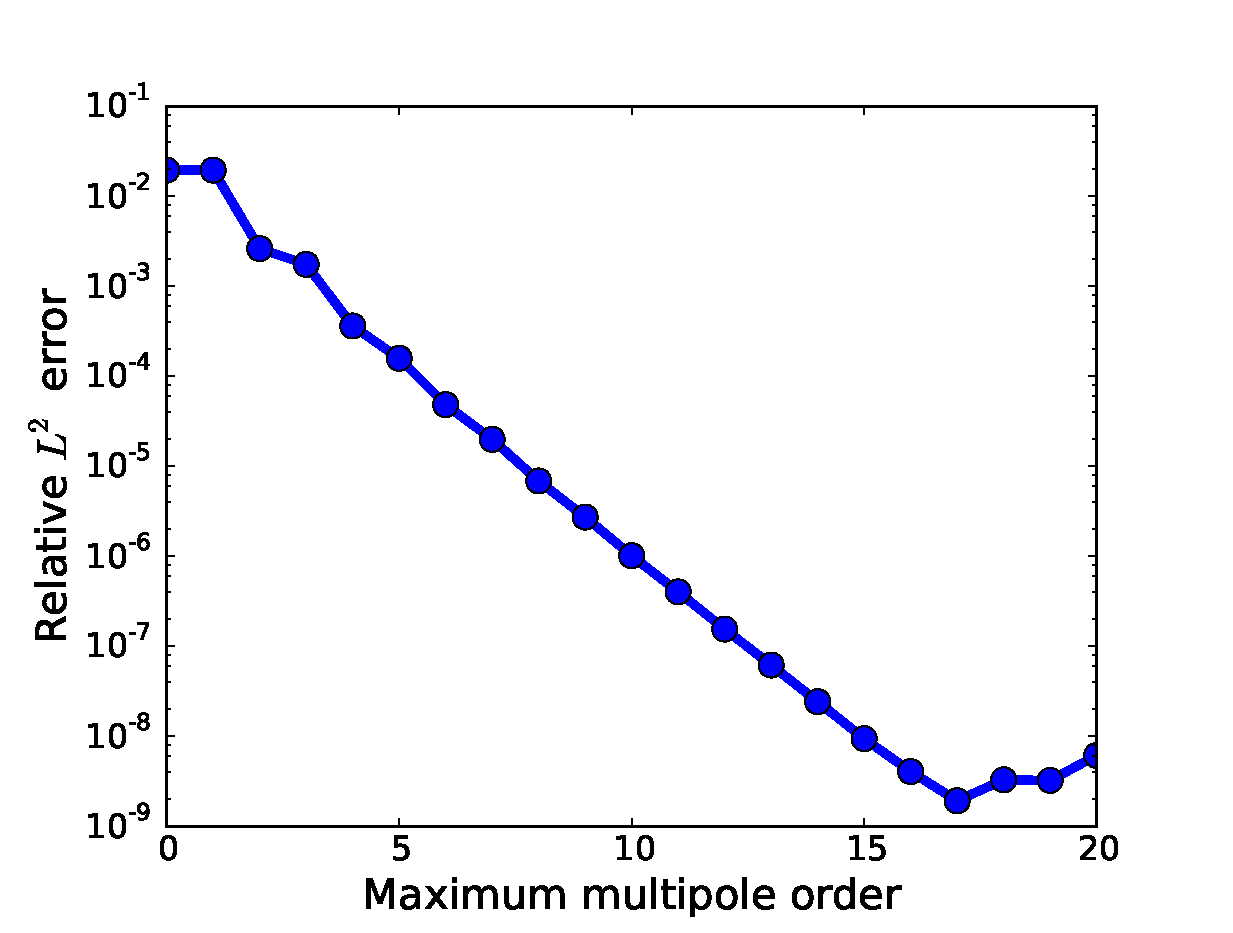
\includegraphics[scale=0.45]{plots/bc_comparison}
  \caption{Error of $\Phi$ on the computational domain for a binary white dwarf simulation 
    whose boundary conditions were computed using various values of the maximum multipole order,
    relative to the exact solution determined by a brute force sum on the boundaries.
    Circles represent the error at integer values, and they have been connected by a smooth 
    line to guide the eye.\label{fig:bc_comparison}}
\end{figure}


\subsubsection{Convergence Testing}\label{sec:gravity_convergence_testing}

Since the results of a merger simulation depend strongly on gravity,
it is important to check whether proper numerical convergence is
achieved for the Poisson solver. To do so, we created a simple test
that inserts a sphere of radius $R$ and uniform mass density $\rho$
onto our grid, and used CASTRO to calculate the gravitational
potential $\Phi$ of this setup. We ensure that $R$ is an integer
multiple of the grid spacing, and the center of the sphere is at the
origin. The problem domain for our simulations is $[-1.6, 1.6]^3$, and
we take $R = 0.5$ and $\rho = 10^3$. The zones with $r > R$ are filled
with an ambient material of very low density. We run this problem at
multiple resolutions corresponding to jumps by a factor of two. For
comparison, at each grid point we evaluate the analytical potential of
a uniform sphere, which can be easily determined using Gauss' law:
\begin{equation}
  \Phi_{\text{sphere}}(r) = -\frac{GM}{r} \times \begin{cases} (3R^2 - r^2)/(2 r^2) & r \leq R \\ 1 & r > R \end{cases},\label{eq:sphere-analytical}
\end{equation}
where $M = 4\pi R^3 / 3$ is the mass of the sphere. We measure the 
numerical error by calculating the $L^2$ norm of the error and 
normalizing it by the $L^2$ norm of the analytical solution:
\begin{equation}
  \text{Error} = \frac{\|\Phi - \Phi_{\text{sphere}}\|_2}{\|\Phi_{\text{sphere}}\|_2}.
\end{equation}

\begin{figure}
  \label{fig:gravity_convergence}
\end{figure}

The results of this test are plotted in Figure
\ref{fig:gravity_convergence}. We find that convergence is actually
substantially better than second-order, and that the difference is
largest at low resolutions. The explanation for this is that we are
attempting to model a spherical object on a rectangular grid. At very
low resolution, the object does not look very spherical. As the
resolution is increased, the total amount of mass on the grid, as well
as its location, will change as the sphere fills out. This means we
are combining the true accuracy bonus from increased resolution with
the artificial accuracy bonus from getting closer to solving the
problem we are supposed to be solving.

We can solve one of these two sources of error by evaluating Equation
\ref{eq:sphere-analytical} with a mass $M$ that corresponds to the
amount of mass actually on the grid, defined as the sum of the density
multiplied by the volume of each cell for all cells that have greater
than ambient density. The resolution study for this case is also
plotted in Figure \ref{fig:gravity_convergence}. We still obtain
convergence better than second-order, indicating that we still have
the geometrical problem.

The only way to fully eliminate this effect is to test a problem that
does not change with resolution. The obvious companion is a cube of
uniform density $\rho$, where now $R$ is half of the side length of
the cube. At each resolution we use the same $R$ as for the sphere,
which ensures that the cube always fills exactly the same fraction of
the domain and thus has the same mass, so the only improvement comes
from better sampling at higher resolution. The potential for this
object has been worked out analytically by \citet{waldvogel:1976} (see
also a similar result in \citealt{hummer:1996}). The potential is in
Equation 15 of that paper, though the last term is missing a factor of
$1/2$, which destroys the symmetry. Inserting this missing factor and
performing a simple coordinate transformation so that the center of
the cube is at the origin, the potential is
\begin{align}
  \Phi_{\text{cube}}(x,y,z) &= -G\rho\sum_{i,j,k=0}^1\left[x_i y_j\, \text{tanh}^{-1}\left(\frac{z_k}{r_{ijk}}\right)\right. \notag \\
  &+ \left. y_j z_k\, \text{tanh}^{-1}\left(\frac{x_i}{r_{ijk}}\right) + z_k x_i\, \text{tanh}^{-1}\left(\frac{y_j}{r_{ijk}}\right) \right.\notag \\
  &\left. - \frac{x_i^2}{2}\,\text{tan}^{-1}\left(\frac{y_j z_k}{x_i r_{ijk}}\right) - \frac{y_j^2}{2}\,\text{tan}^{-1}\left(\frac{z_k x_i}{y_j r_{ijk}}\right) \right. \notag \\
  &- \left. \frac{z_k^2}{2}\,\text{tan}^{-1}\left(\frac{x_i y_j}{z_k r_{ijk}}\right)\right]
\end{align}
where $x_0 = R + x$, $x_1 = R - x$, $y_0 = R + y$, $y_1 = R-y$, $z_0 =
R+z$, $z_1 = R-z$, and $r_{ijk} = \sqrt{x_i^2 + y_j^2 + z_k^2}$. In
\texttt{FORTRAN} and \texttt{C}, the inverse hyperbolic tangent is
\texttt{atanh} and the inverse tangent is \texttt{atan} (\textit{not}
\texttt{atan2}). This formula is valid both inside and outside the
cube. The normalized $L^2$ error norm for this problem is also shown
in Figure \ref{fig:gravity_convergence}, and indeed we see
near-perfect second-order scaling.

The main lesson here is that in a convergence study, it is important
to ensure that the physical problem does not change with
resolution. Since in the case of spherical objects on rectangular
grids the effect is to artificially boost convergence with resolution,
in a simulation with spherical objects like stars one can envision a
scenario of being fooled into believing apparently good convergence
results that are simply a convolution of artificially high
gravitational convergence and poor convergence in the hydrodynamics. A
convergence study in this case is only fully valid if there is reason
to be confident that this effect is negligible compared to other
factors.

Another factor that may affect convergence testing is easily seen in
Figure \ref{fig:gravity_convergence}, where at the highest resolution
the error flattens out. This occurs because of a limitation in the
accuracy of the multigrid solver. For problems of this size we find
empirically that the multigrid solver does not converge for error
tolerances smaller than about $10^{-11}$, which enforces a lower limit
on the total error. This is also something to be aware of in assessing
convergence for our full simulations.

\subsection{Rotation}\label{sec:rotation}

For the evolution of binary systems, it is most natural to evolve the
two stars in a frame that is co-rotating at the same period as the
orbital period. Since the publication of the original code paper, CASTRO 
now has the ability to evolve systems in a rotating reference frame. 
Source terms corresponding to the Coriolis and centrifugal 
force terms are added to the momentum and energy equations. In this frame, 
the stars essentially remain stationary in their original positions due to the
centrifugal force supporting against the gravitational attraction, and
will remain this way as long as significant mass transfer does not
occur. \cite{swc:2000} demonstrated (in the context of neutron star
mergers) that conservation of angular momentum is much easier to
obtain in the rotating reference frame than in an inertial frame in
which stars advect large amounts of material around the domain. We
wish to emphasize that although it is commonly stated in the
literature that grid-based codes poorly conserve angular momentum,
it is only generally true that grid-based codes do not exactly conserve 
angular momentum when the equations are written in conservative form
for linear momentum. (See also \cite{motl:2002} for an example of how 
to evolve the hydrodynamics equations for angular momentum.) 
The extent to which angular momentum conservation is violated
will be a function of the resolution. When this is sufficiently high
and a rotating reference frame is employed, excellent conservation
properties can result, as demonstrated in Section \ref{sec:kepler}. 
In particular, at reasonable resolution for a binary orbit our code 
conserves angular momentum well enough that this no longer becomes 
a reason to use a Lagrangian method such as smoothed-particle hydrodynamics.
We note that as the stars begin to coalesce, the rotating reference frame
will no longer provide a good approximation to the spatial motion of
the stars and then they will begin to significantly move around the
domain. This is not necessarily problematic because the most important
feature of the rotating frame is that it helps ensure that the initial
coalescence is not the result of spurious numerical loss of angular
momentum. When significant mass transfer sets in and evolution
proceeds on a dynamical timescale, the conservation properties may be
slightly worse but angular momentum conservation is also less
important.

In a rotating reference frame with angular frequency vector $\bm{\omega}$, the momentum equation becomes:
\begin{equation}
  \left.\frac{\partial(\rho \mathbf{u})}{\partial t}\right|_{\text{rot}} = -2\, {\bm\omega} \times (\rho\mathbf{u}) - \rho {\bm\omega} \times \left({\bm\omega} \times \mathbf{r}\right).
\end{equation}
Here $\mathbf{r}$ is the position vector with respect to the origin. Typically we choose $\bm{\omega} = (0, 0, 2\pi / T)^T$,
with the rotation axis coincident with the $z$ axis at $x = y = 0$.
$T$ is the rotation period, which is the most natural quantity to specify
for a rotating stellar system. As described in the appendix, we include this source term
in the edge state prediction in a way that is analogous to the gravity source.
We evaluate all quantities at cell centers and use the same predictor-corrector 
approach that we use for the gravity source terms to the momentum equations.

The update to the energy equation can be determined by taking the dot product of the velocity
with the momentum source terms. The Coriolis term vanishes identically, as it must
because the Coriolis term does no work on the fluid. The update from the centrifugal force becomes
\begin{equation}
  \left.\frac{\partial(\rho E)}{\partial t}\right|_{\text{rot}} = \frac{1}{\Delta V}\int \rho \mathbf{u} \cdot \mathbf{f}_R\, dV,
\end{equation}
with $\mathbf{f}_R \equiv  -{\bm\omega} \times \left({\bm\omega} \times \mathbf{r}\right)$. 
This expression is identical to the gravity source under the interchange of $\mathbf{g}$ with $\mathbf{f}_R$.
As observed by \cite{marcello:2012}, we can similarly write down a rotational potential,
\begin{equation}
  \Phi_R = -\frac{1}{2} \left| {\bm\omega} \times \mathbf{r} \right|^2.
\end{equation}
Therefore we can retrace the steps of Section \ref{sec:gravity_hydro_coupling} to obtain
an update to $(\rho E)$ that conserves the total energy in the presence of rotation,
\begin{equation}
  (\rho E_{\text{tot}}) = (\rho E) + \frac{1}{2} \rho \Phi + \rho \Phi_R.
\end{equation}
In one dimension, this would be
\begin{align}
  \left.\Delta(\rho E_i)\right|_{\text{rot}} &= \frac{1}{2} \Delta m_{i-1/2} (\Phi_{R_{i}} - \Phi_{R_{i-1}}) \notag \\
  &+ \frac{1}{2} \Delta m_{i+1/2} (\Phi_{R_{i+1}} - \Phi_{R_{i}}).
\end{align}
As with gravity, in three dimensions we include the mass fluxes through all six cell faces.

We apply the rotation forces after the gravitation forces, but 
there is some freedom in the order in which to apply the gravitational and rotational terms.
This order may matter because the Coriolis force depends on the fluid velocity, and 
in the predictor-corrector approach, we use the velocities both at 
time-level $n$ and time-level $n+1$. If we update the latter with the gravitational force, 
then the Coriolis force will see a different velocity than the one obtained through the 
pure hydrodynamics step. (This does not matter for the energy equation in our new formulation,
because the velocities used are always the time-level $n+1/2$ values coming from the Riemann solver.)
In practice, this will not matter significantly for our simulations in this work 
because the centrifugal force plays the dominant role in maintaining stability of non-contact 
binary systems, and the centrifugal force does not depend on the fluid velocity.
However, this issue may be worth exploring in future work in situations where the Coriolis 
term is non-negligible in determining the system evolution.

In all simulations performed in a rotating reference frame, we will transform all relevant
quantities back to the inertial reference frame when reporting them in this paper. In particular,
for every zone we add to the displayed kinetic energy the rotational energy associated with motion 
at the circular velocity corresponding to the distance of that zone from the rotation axis.
We do the analogous calculation for angular momentum as well. When plotting the locations of 
stars on the grid, we rotate them by an angle corresponding to the amount of time that has 
passed since the simulation started.

%==========================================================================
% Initial Models and Problem Setup
%==========================================================================

\section{Initial Models and Problem Setup}
\label{sec:initial_models}

At the start of any full simulation, we generate initial model white
dwarfs by integrating the equation of hydrostatic equilibrium, taking
the temperature and composition to be constant, and using the general
stellar equation of state.  This results in a single non-linear
equation to find the density in a zone given the conditions in the
zone beneath it:
\begin{equation}
\frac{p_{i+1} - p_i}{\Delta x} = \frac{1}{2} (\rho_i + \rho_{i+1}) g_{i+1/2}.
\end{equation}
This equation is a function of $\rho_{i+1}$ only since the pressure is
uniquely determined by the density in this case. Here, $\rho_i$ and $p_i$
are known, $g_{i+1/2}$ is the gravitational acceleration at the
interface between zones $i$ and $i+1$, found by simply adding up all
the mass from zones $1, \ldots, i$ to get the enclosed mass,
$M_{i+1/2}$, and then setting $g_{i+1/2} =
-GM_{i+1/2}/r_{i+1/2}^2$. We solve this equation for $\rho_{i+1}$
using a Newton-Raphson iteration.

We desire to specify the mass of the white dwarf, as well as its
temperature and composition. To start the integration off, we
therefore need to guess at a central density.  We then do a secant
iteration over the entire integration procedure to find the central
density needed to yield the desired total mass.  We note that the grid
spacing $\Delta x$ is chosen such that it is equal to the zone size on
the finest level of our problem, which is known in advance since we
specify the domain size and the maximum number of possible levels of
refinement.

We map the 1D model onto the 3D Cartesian grid by taking density,
temperature, and composition as the independent variables,
interpolating these to the cell centers, and then calling the equation
of state to initialize the remaining terms.  The interpolation process
divides each zone into $n_{\text{sub}}$ sub-zones of equal volume for
the purpose of sampling the 1D model, and the sub-zones are added
together to obtain the full zone's characteristics. This
sub-grid-scale interpolation is useful near the edge of the star,
where the density falls off rapidly with radius.

For a single star simulation, the star is simply placed at the center
of the computational domain, which we take to be the origin. For a
binary star simulation, we take as parameters the mass of the two
white dwarfs and the initial orbital period $T$. Using Kepler's third
law and assuming a circular orbit, we can then work out the orbital
separation $a$:
\begin{equation}
  a = \left(\frac{GM T^2}{4\pi^2}\right)^{1/3}.
\end{equation}
Here $M = M_P + M_S$ is the total mass of the system, where $M_P$ is
the specified \textit{primary} mass and $M_S$ is the specified
\textit{secondary} mass. The primary WD will always start on the left
side of the computational domain for our simulations, and is more
massive than the secondary. This reflects the usual terminology in the
literature where the primary WD is the accretor and the secondary is
the donor. The center of mass is located at the center of the
computational domain, and the stars lie along the $x$ axis, so that
the primary's center of mass is located at $x = -(M_S / M)\, a$ and
the secondary's center of mass is located at $x = (M_P / M)\, a$.

The initial velocity is taken to be zero in if we are in the reference
frame that rotates with the WDs, and if we are in the inertial frame
the velocity is set equal to the rigid rotation rate corresponding to
the specified period $T$.

We do not attempt to enforce equilibrium with an additional relaxation
step. This will be an important part of future work in this series, as
numerous groups working on binary evolution
\citep{swc:2000,motl:2002,rosswog:2004,dan:2011,pakmor:2012:gadget}
have commented on the importance of equilibrium initial conditions in
determining the evolution of the system. In particular, we plan to
compare the self-consistent field method (which finds an equilibrium
solution \textit{a priori}) and the method of \cite{rosswog:2004},
which starts with our method and then attempts to guide the evolution
toward the equilibrium state using suitably defined damping
terms. However, these issues are not considered for the present study,
as we are not yet attempting to study the merger process.

As a consequence of starting in a non-equilibrium setting, there are 
large density and pressure gradients near the white dwarf surfaces
that result in large amounts of mass flowing into the ambient
medium. This can result in spurious non-physical consequences such as 
the total density or energy going negative in a zone. To compensate 
for this, we start the simulation with a timestep that is a few orders 
of magnitude smaller than that required by the CFL criterion, and allow
the timestep to increase by 1\% each timestep so that the timestep reaches 
its maximum allowed by the velocities on the grid over a span of approximately 
1000 timesteps. This allows the ambient medium just outside the white dwarf
to come closer to equilibrium with the surface without having 
discontinuous jumps in the density or energy. For all simulations, 
the maximum timestep is set to be equal to one-half of the CFL limit.

We track a number of diagnostic quantities at the end of every coarse grid timestep. 
For all simulations, we record the total energy (including the breakdown into
its components: kinetic, internal, gravitational potential, rotation; we note
that for the diagnostics we actually use $(\rho E)$ for calculation of the total energy,
rather than explicitly calculating the sum of kinetic and internal, as this is
the quantity that should be explicitly conserved), 
the total angular momentum, and the center of mass of the system. 
For stellar calculations, we separately record diagnostic 
information about the stars, including their centers of mass, 
and the volume contained within each star.

The software used to generate the test problems in this paper
(as well as the manuscript itself),
\texttt{wdmerger}\footnote{\url{https://github.com/BoxLib-Codes/wdmerger}},
is freely available at an online repository hosting service.
Version control in both the parent software (BoxLib, CASTRO) and in \texttt{wdmerger}
permits us to reference the state of the code at the time a simulation
was performed. In all plot files and diagnostic output generated by CASTRO, 
and EPS figure files and plots generated by \texttt{wdmerger} for this work,
we store the active \texttt{git} commit hashes of BoxLib, CASTRO and \texttt{wdmerger}.

%==========================================================================
% Numerical Test Problems
%==========================================================================
\section{Numerical Test Problems}\label{sec:Tests}

Merger simulations face a number of numerical difficulties that are
not present in single-degenerate Type Ia and core-collapse supernova
simulations. In Section \ref{sec:gravity}, we discussed how the lack
of spherical symmetry necessitates a careful look at the gravity
solver. There are also hydrodynamical issues: the merger process will
result in substantial motion of stellar material across the grid. This
bulk motion presents an opportunity for advection errors to build up,
and is only partially mitigated by evolving the white dwarfs in a
co-rotating frame. It is therefore important to be be aware of the
behavior of the code in such circumstances. The behavior of CASTRO for
many standard hydrodynamics test problems was detailed in the original
code paper \citep{castro}, and in the interest of brevity we will not
repeat them here. Instead, we focus on a subset of problems that
highlight the special difficulties introduced in merger
simulations. These problems couple the hydrodynamics, gravity and
equation of state modules. We observe that while in most non-trivial
three-dimensional problems this creates a complexity that makes it
impossible to determine exact analytical solutions, it is
straightforward to devise problems for which certain global properties
should obey simple, expected behaviors. Where possible, these should
be quantified and a convergence study performed. We recommend that all
simulation codes should check their performance on such problems to
ensure their reliability when coupling the various physics modules
necessary to build a complete and realistic simulation.

\subsection{Maintaining Hydrostatic Equilibrium}\label{sec:HSE}

In Section \ref{sec:initial_models} we describe the process by which
we generate initial stellar models. While the 1D models are in
hydrostatic equilibrium to within a small error, interpolation onto
the 3D Cartesian grid will introduce perturbations into the solution
\citep{zingale:2002}. Although we ensure that the initial models are
generated with the same equation of state and are as well resolved as
our finest grid, there will still be a hydrodynamical error associated
with the fact that the rectangular grid cannot faithfully represent a
spherical star. Additionally, the gravitational potential obtained by
the multigrid solver will differ slightly from the one assumed by the
initial model, and the operator splitting between the gravity and
hydrodynamics should also result in small errors. As a result, we
expect that the star will oscillate slightly about an equilibrium
point, but that the amplitude of this oscillation should decrease with
increasing resolution.

This problem was studied in the first CASTRO paper, but is worth
revisiting here. A single star explosion simulation may only last a
couple of seconds, and the CASTRO paper studied the behavior of the
star after one second of evolution. However, the dynamical timescale
of a typical carbon-oxygen white dwarf is on the order of 1--10
seconds. Additionally, a binary orbit is typically on the order of
10--100 seconds when a merger simulation starts, and with equilibrium
initial conditions the system may survive for tens of orbits before
the secondary is disrupted. When this does happen, we want to be
confident that it was because of the dynamics of the merger process
and not because of an instability in an individual star. Our goal here
is thus to populate a single star onto our three-dimensional
coordinate grid and evolve it for a period of time long enough to
assess whether the star is truly stable, and to probe how the size of
deviation from equilibrium is affected by grid resolution.

\subsection{Gravitational Free Fall}\label{sec:Gravitational Free Fall}

A simple dynamical test to verify the gravitation physics in CASTRO is
the case of gravitational free fall. We place two stars on the grid 
in the manner of Section \ref{sec:initial_models}. The distance $a$ between 
them corresponds to a chosen orbital period $T$, consistent with the total
system mass $M$, but we disable the rotational source terms so that 
the stars start at rest in an inertial reference frame. 
Thus the stars will simply begin moving toward each other.
As long as the stars remain approximately spherical, the stars can be 
treated as point masses (this only seriously breaks down after the stars
have come into contact). In dimensionless units where $r \to r / a$ and 
$t \to 2\sqrt{2}\pi t / T$, the simple free fall equation of motion governing the
distance $r$ between their centers of mass takes the form:
\begin{equation}
  \ddot{r}(t) = - \frac{1}{2r^2}.
\end{equation}
It is possible to derive a closed-form solution for the evolution time
as a function of separation by starting with the integral formulation,
\begin{equation}
  t(r) = \int_{1}^{r} \frac{dr}{v(r)}.
\end{equation}
The velocity $v$ (in dimensionless units) can be found by noting that 
$\ddot{r} = v\, dv / dr$ and then separating and integrating the equation 
of motion. This yields 
\begin{equation}
  v(r) = \sqrt{\left(\frac{1}{r} - 1\right)}.
\end{equation}
For our problem $0 \leq r \leq 1$, so this is always valid. Integrating, we find
\begin{equation}
  t(r) = \text{arccos}\left(\sqrt{r}\right) + \sqrt{r \left(1 - r\right)}. \label{analyticalFreeFall}
\end{equation}
so that the point of contact would occur at $t = 1$. We actually stop the simulation
at $t = 0.9$, which is when the effects from the extended sizes of the stars
starts to become important. The results of our simulation for our default $256^3$ zone 
uniform grid are shown in Figure \ref{Fig:Free Fall}. They show excellent agreement
between the theory and the simulation results, and this agreement holds even for 
a more moderate $128^3$ zone simulation.

\begin{figure}
  \centering
  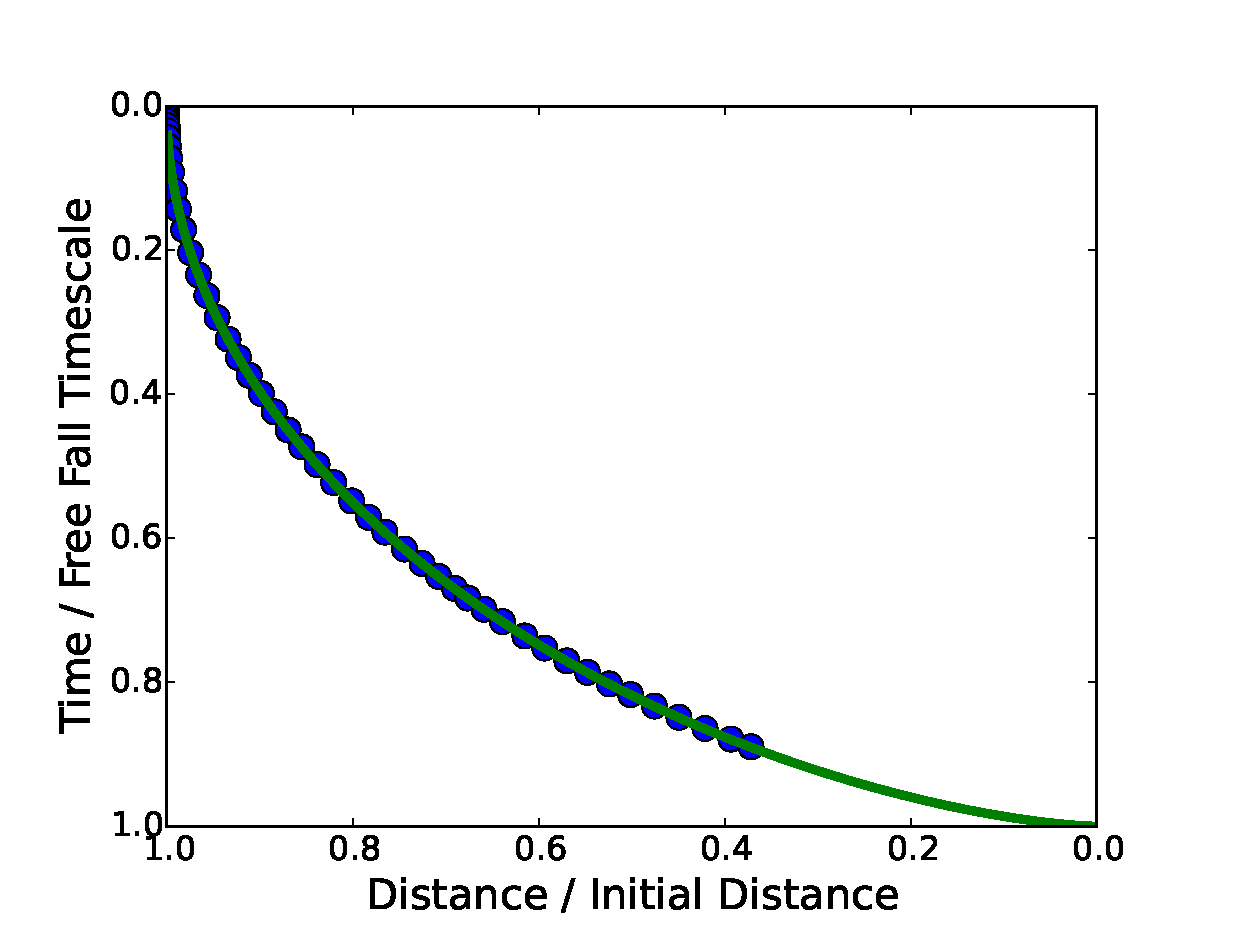
\includegraphics[scale=0.45]{plots/freefall}
  \caption{Time evolution of two initially stationary white dwarfs,
    mutually attracted to each other by the gravitational force. The
    horizontal axis gives the separation of the white dwarfs, scaled
    to the initial separation, and the vertical axis gives the elapsed
    time of the simulation, scaled to the time it would take two point masses
    to collide. The solid curve shows the analytical result,
    calculated from Newtonian mechanics, and the circles show the
    samples from the time evolution with CASTRO. For visual clarity, we 
    show only a small fraction of the timesteps.}
  \label{Fig:Free Fall}
\end{figure}

\subsection{Galilean Invariance}\label{sec:galileo}

It is often stated in the literature that Eulerian methods for
hydrodynamics with grids fixed in space do not obey the Galilean
invariance of the underlying Euler equations, so that simulations
moving at a uniform bulk velocity will appear different than an
equivalent stationary simulation. If true, this means that codes such
as CASTRO may be fundamentally inappropriate for merger problems
(though any errors should be greatly diminished in a reference frame
that rotates with the initial binary orbit). Recently, this has come
up in two ways which are of note for us in the present study. We will
explain these situations and run tests to determine whether this
actually is a significant concern.

\citet{arepo} performed a Kelvin-Helmholtz instability test and showed
that (at low resolution) a fixed-grid code failed to develop the
expected fluid instability when the whole fluid was moving at a
strongly supersonic uniform velocity. This contrasted with the results
of the moving-mesh code AREPO being presented in that study, which
demonstrated Galilean invariance even at large bulk velocities. If
verified, this claim would have important consequences on how much we
can trust the ability of CASTRO to test the violent merger progenitor
model. Shearing between the material flowing out of the secondary and
material near the surface of the primary may trigger fluid
instabilities that play an important role in the evolution of that
gas, which is the site of the initial detonation in the prompt
explosion model. \citet{guillochon:2010} showed for their simulation
that Kelvin-Helmholtz instabilities produced this way may raise the
temperature of the accreting material enough to ignite a
detonation. Therefore if we are not correctly reproducing the
characteristics of the Kelvin-Helmholtz instability in the case where
there is significant mass motion on the grid, we cannot be confident
that a detonation (or lack thereof) is not numerically
seeded. However, \citet{robertson:2010} observe that Galilean
invariance of simulation results for the Euler equations occurs only
because of truncation error in the discretization of the fluid
equations. This takes the form of a numerical diffusion term which is
dependent on velocity (and also resolution). The advantage of a
moving-mesh code is that the mesh everywhere moves with the local flow
velocity, which substantially reduces the numerical
diffusion. \citeauthor{robertson:2010} argue that the differences seen
between the moving-mesh and fixed-grid code are caused by the
interaction of this numerical diffusion with small-scale instabilities
(which may be physical or numerical) which couple with and
fundamentally alter the large-scale modes. Small-scale instabilities
are seeded in this problem by the choice of a sharp initial
discontinuity between the fluids. Crucially though,
\citeauthor{robertson:2010} point out that this problem does not
converge with resolution and so it is not possible to know the correct
behavior of this problem. As such, we do not know whether the
small-scale modes found in AREPO are real, so the problem is not
useful in formally discriminating between methodologies. They instead
propose an alternate test with a smoother initial contact. This
converges to the same solution qualitatively in both the stationary
and bulk velocity cases, indicating that the code does generally
maintain Galilean invariance (to some specified error that depends on
resolution and the uniform flow speed).  We will see whether we can
reproduce this result, as well as a result by \cite{wadsley:2008}, who
used the FLASH code to simulate a hot bubble subject to mixing by the
Kelvin-Helmholtz instability, and also found that the mixing was
affected by a uniform bulk velocity.

A related question is whether our code reliably simulates the bulk
motion of the stars across the grid, and whether such bulk motion
affects the stability of the star. This concern is prompted by the
study of \cite{tasker:2008}, who studied the effect of uniform
translation on the stability of a spherically symmetric model for a
galaxy cluster. They compared the radial profile of the cluster at
initialization and after a period of time evolution. Using FLASH and
ENZO, they found that a static cluster retains its shape at high
enough resolution, while uniform translation of the cluster causes
mixing of the core material due to numerical diffusion which results
in an underestimation of the core's true density. The SPH codes they
used did a better job maintaining the core density. We will perform a
variant of this test using white dwarf models.

\subsubsection{Kelvin-Helmholtz Instability}\label{sec:khi}

Following \cite{robertson:2010}, we set up a Kelvin-Helmholtz test in
the following way. The problem domain runs from 0 to 1 in both the $x$
and $y$ directions. Though this is a two-dimensional test, we run
CASTRO in 3D and replicate the problem along 8 cells in the $z$
direction; the physical size of these zones is determined so that $dz
= dx = dy$, a requirement at present in CASTRO. The problem involves a
fluid slab of density $\rho_1 = 2.0$ traveling rightward in the
$x$-direction at velocity $v_1 = 0.5$, sandwiched by a fluid of
density $\rho_2 = 1.0$ traveling leftward at velocity $v_2 =
-0.5$. The density gradient is in the $y$ direction, so this creates a
velocity shear along the interface between the fluids. The density and
velocity distribution on the computational domain are given by:
\begin{align}
  \rho &= \rho_1 + R(y)\left[\rho_2 - \rho_1\right] \\
  v_x  &= v_1 + R(y)\left[v_2 - v_1\right] \\
  v_y  &= v_{\text{bulk}} + v^\prime
\end{align}
Here $R(y)$ is a ramp function that describes the transition between
the two fluids, while $v_{\text{bulk}}$ is the bulk motion of the
fluid in the $y$ direction and $v^\prime$ is the velocity perturbation
that seeds the instability. The problem will be established for two
sets of initial conditions (ICs), which we follow
\citeauthor{robertson:2010} in calling ICs A and B. They differ in
their ramp function ($R_A$ and $R_B$ respectively), as well as the
initial perturbation ($v^\prime_A$ and $v^\prime_B$ respectively), and
the frequency of the perturbation ($n_A = 4$ and $n_B = 2$):
\begin{align}
  R_A &= \begin{cases} 0 & |y - 0.5| > 0.25 \\ 1 & |y - 0.5| < 0.25 \end{cases} \\
  R_B &= \Big\{\left[1 + e^{-2(y-0.25)/\Delta_y}\right]\left[1 + e^{2(y-0.75)/\Delta_y}\right]\Big\}^{-1} \\
  v^\prime_A &= w_0\, \text{sin}\left(n_A\, \pi\, x\right) \left\{e^{-(y-0.25)^2 / 2\sigma^2} + e^{-(y-0.75)^2/2\sigma^2}\right\} \\
  v^\prime_B &= w_0\, \text{sin}\left(n_B\, \pi\, x\right).
\end{align}
Here $w_0 = 0.1$ is the scale of the velocity perturbation, $\sigma =
0.05/\sqrt{2}$ controls the width of the Gaussian for IC A, and
$\Delta_y$ is the transition distance scale for the smooth ramp of IC
B. The pressure everywhere is set to $p = 2.5$, and we run this with a
gamma-law equation of state set to $\gamma = 5/3$. Plotfiles are
generated every 0.01 seconds, and the problem is run until $t = 2$.

We run the problem for $v_\text{bulk} = [0, 1, 3, 10, 30, 100]$, and
for each set of initial conditions run the problem at resolutions of
$64^2$, $128^2$, $256^2$, $512^2$. In addition, for each initial
condition we run a simulation at the very high resolution of $2560^2$
for the stationary problem only. This serves as a reference solution
to gauge the extent to which the bulk flow affects the development of
the fluid instability.

\subsubsection{Hot Bubble}\label{sec:hot_bubble}

\subsubsection{Moving Star}\label{sed:moving_star}

\subsection{Keplerian Orbit}\label{sec:kepler}

should show:

effect of resolution

inertial vs. rotating frame

effect of ppm\_reference and gravity update type

effect of boundary conditions (size of domain and possibly multipole dependence)


%==========================================================================
% Performance
%==========================================================================
\section{Performance}\label{sec:Performance}

strong scaling plot

space filling curve?

OMP vs. MPI?

breakdown by component?


%==========================================================================
% Conclusions
%==========================================================================
\section{Conclusions and Discussion}\label{sec:Conclusions and Discussion}


\acknowledgments

The authors thank Noel Scudder and Platon Karpov for their help with 
this project, especially related to visualization of the results. 
We also thank Adam Jacobs for his advice on and assistance with 
running on supercomputing resources.

This research was supported by NSF award AST-1211563. An
award of computer time was provided by the Innovative and Novel
Computational Impact on Theory and Experiment (INCITE) program.  This
research used resources of the Oak Ridge Leadership Computing Facility
located in the Oak Ridge National Laboratory, which is supported by
the Office of Science of the Department of Energy under Contract
DE-AC05-00OR22725. Projects AST006 and AST106 supported use of the ORNL/Titan resource. 
This research is part of the Blue Waters sustained-petascale computing project, 
which is supported by the National Science Foundation (awards OCI-0725070 
and ACI-1238993) and the state of Illinois. Blue Waters is a joint 
effort of the University of Illinois at Urbana-Champaign and its 
National Center for Supercomputing Applications.
This research used resources of the National Energy Research Scientific Computing
Center, which is supported by the Office of Science of the
U.S. Department of Energy under Contract No. DE-AC02-05CH11231.  
This work used the Extreme Science and Engineering Discovery Environment (XSEDE), 
which is supported by National Science Foundation grant number ACI-1053575. 
Project AST100037 supported use of the resources NICS/Kraken and NICS/Darter.

\clearpage

\bibliographystyle{../apj}
\bibliography{../refs}


\clearpage
\appendix

\section{CASTRO hydrodynamics changes}

The basic PPM algorithm in CASTRO has undergone a number of changes
since the original code paper \citep{castro}.  A discussion of the
pure hydrodynamics changes along with verification of CASTRO when
using the stellar equation of state was given in
\citet{zingalekatz:2015}.  Here we discuss the changes that affect
multispecies flow and source terms.

Summary of changes:
\begin{itemize}
\item New gravity update type: fixes some energy conservation

\item changing I's to use limit of the parabola instead of the
  cell-center: not sure if this does much

\item Colella \& Glaz Riemann solver: does a much better job with
  temperature in strong shocks

\item Tracing of gravity: seems to help with the material at the edge
  of the star

\item implicit update of the rotation terms?  (I coded this up once, but
  it is not currently in the code)
\end{itemize}

\subsection{Reference States}

For all the runs, the PPM reconstruction is done using the original limiters for
the parabolic profiles \citep{ppm}.  The prediction of the interface
states appears as:
\begin{equation}
\label{eq:ppmstatel}
q_{i+1/2,L}^{n+1/2} = \tilde{q}_L -
   \sum_{\nu;\lambda_i^{(\nu)}\ge 0} l_i^{(\nu)} \cdot \left [
        \tilde{q}_L  - \mathcal{I}^{(\nu)}_+(q_i)
       \right ] r_i^{(\nu)}
\end{equation}
where $q$ is the vector of primitive variables, $l_i^{(\nu)}$ and
$r_i^{(\nu)}$ are the left and right eigenvectors with eigenvalue
$\lambda_i^{(\nu)}$, with $\nu$ the index of the characteristic wave of
the system.  The sum is over all the waves that result from the
characteristic structure of the problem, but designed such that only
waves moving toward the interface contribute to the interface value,
$q_{i+1/2,L}^{n+1/2}$.  The reference state, $\tilde{q}_L$ is
chosen to minimize the work of the characteristic projection.
Finally, $\mathcal{I}_+^{(\nu)}(q)$ is the
average under the parabolic profile of quantity $q$ of all the
information that can reach the right interface of the zone $i$ as
carried by the wave $\nu$.  The reader is referred to
\citet{ppmunsplit} for further defaults.

Since the original CASTRO paper, the reference state implementation
has been switched to:
\begin{equation}
\label{eq:refchoice}
\tilde{q}_L = \left \{ \begin{array}{cc}
       \mathcal{I}_+^{(+)}(q_i) & \mathrm{if~} u + c > 0 \\
       q_i                    & \mathrm{otherwise}
\end{array}
\right .
\end{equation}
where the $(+)$ superscript here means the fastest wave moving to the right
(the $u+c$ eigenvalue).   This is simply the average under the largest
portion of the parabolic profile that could possible reach the interface 
over the timestep.  This is
in agreement with \citet{ppmunsplit} (eq. 90).  The flattening
in the original CASTRO paper has also been updated as discussed
in \citet{zingalekatz:2015}.

We comment on the choice of reference state for passively-advected
quantities (like $X_k$ or the transverse velocity).
First, consider one of the variables present in one-dimensional flow
(density, velocity in the normal direction, and pressure).  Here we
our reference state is as in Eq.~\ref{eq:refchoice} and we have.
Ignoring flattening, if there are no waves moving toward our
interface, then Eq.~\ref{eq:ppmstatel} reduces to:
\begin{equation}
q_{i+1/2,L}^{n+1/2} = \tilde{q}_L = q_i
\end{equation}
If instead only the fastest wave is moving toward the interface, then
only the term corresponding to the fastest wave in the sum will be
added in Eq.~\ref{eq:ppmstatel}, but our choice of reference state makes
that term 0 by design, and our interface state is:
\begin{equation}
q_{i+1/2,L}^{n+1/2} = \tilde{q}_L = \mathcal{I}_+^{+}(q_i)
\end{equation}
This is the desired behavior for each of these cases. 

The details of the reference state for passively advected quantities 
(which includes the transverse velocities in the 1-d tracing) is not
typically discussed.  If we use the same idea of the reference state as
in Eq.~\ref{eq:refchoice}, and consider a quantity $\xi$ which should only
jump across the contact, then our interface state becomes:
\begin{equation}
\xi_{i+1/2,L}^{n+1/2} = \tilde{\xi}_L -
  \underbrace{l_i^\evz \cdot \left [
        \tilde{\xi}_L  - \mathcal{I}^\evz_+(\xi_i)
       \right ] r_i^\evz}_{\text{only if~$u \ge 0$}}
\end{equation}
Again, ignoring flattening, if $u \ge 0$, then we have
\begin{equation}
\xi_{i+1/2,L}^{n+1/2} = \tilde{\xi}_L -
  \left (\tilde{\xi}_L  - \mathcal{I}^\evz_+(\xi_i) \right ) = \mathcal{I}^\evz_+(\xi_i)
\end{equation}
(where we used the fact that the eigenvectors are normalized to 1 and
don't mix in any other states when dealing with passive terms).  This
is the expected behavior---we see a state that is traced only by the
contact wave.  However, if $u < 0$ but $u + c \ge 0$, then we instead get:
\begin{equation}
\xi_{i+1/2,L}^{n+1/2} = \tilde{\xi}_L = \mathcal{I}^\evp_+(\xi_i)
\end{equation}
Here we used the same definition of the reference state and see that our
interface state sees the profile traced under the fastest wave, not the
contact.  This is not the correct behavior for a passively-advected
quantity.  

The fix for passively-advected quantities is to simply ignore the 
idea of a reference state and just test on the speed of the contact
itself, setting:
\begin{equation}
\xi_{i+1/2,L}^{n+1/2} = \left \{ \begin{array}{cc}
       \mathcal{I}_+^\evz(\xi_i) & \mathrm{if~} u  > 0 \\
       \xi_i                    & \mathrm{otherwise}
\end{array}
\right .
\end{equation}



\subsection{Gravity and Rotation Tracing}

We note a few additional differences between the original PPM
implementation of \citet{ppm} and CASTRO.  In the original PPM
implementation, the gravitational acceleration was reconstructed as a parabola, and
this was traced under to find the forcing that affects the interface
for each wave.  CASTRO followed \citet{ppmunsplit} which instead adds
$(\Delta t/2)g$ to the interface states at the end of the
reconstruction.  In the current implementation, we do the original
parabolic reconstruction and characteristic tracing of the gravitation
source.  Our system with the source appears as:
\begin{equation}
q_t + A(q) q_x = G
\end{equation}
where $G = (0, g, 0)^T$---i.e. the gravitational source only affects
$u$, not $\rho$ or $p$.  Note that in the PPM paper, they put $G$ on 
the lefthand side of the primitive variable equation, so our signs are
opposite.  Our projections are now:
\begin{equation}
\sum_{\nu; \lambda^\enu \ge 0}l^\enu \cdot (\tilde{q} - \mathcal{I}^\enu_+(q) - \tfrac{\Delta t}{2} G) r^\enu
\end{equation}
for the left state, and
\begin{equation}
\sum_{\nu; \lambda^\enu \le 0} l^\enu \cdot (\tilde{q} - \mathcal{I}^\enu_-(q) - \tfrac{\Delta t}{2} G) r^\enu 
\end{equation}
for the right state.  Since $G$ is only non-zero for velocity, only
the velocity changes.  Writing out the sum (and performing the vector products), we
get:
\begin{eqnarray}
u_{i+1/2,L}^{n+1/2} =
   \tilde{u}_+ 
  &-& \frac{1}{2} \left [
      \left (\tilde{u}_+ - \mathcal{I}_+^\evm(u) - \frac{\Delta t}{2} \mathcal{I}^\evm_+(g) \right ) - 
       \frac{\tilde{p}_+ - \mathcal{I}_+^\evm(p)}{C} \right ] \nonumber \\
  &-& \frac{1}{2} \left [
      \left (\tilde{u}_+ - \mathcal{I}_+^\evp(u) - \frac{\Delta t}{2} \mathcal{I}^\evp_+(g) \right ) +
       \frac{\tilde{p}_+ - \mathcal{I}_+^\evp(p)}{C} \right ]
\end{eqnarray}
These differ from the expression in the PPM paper, where $\Delta t G$,
not $\Delta t/2 G$ is used in the projection, however we believe that
the factor of $1/2$ is correct.  To see this, notice that if both
waves are moving toward the interface, then the source term that is
added to the interface state is $(\Delta t/4) (\mathcal{I}_+^\evm(g) +
\mathcal{I}_+^\evp(g))$ for the left state, which reduces to $(\Delta
t/2) g$ for constant g---this matches the result from Taylor
expanding to the interface at the half-time (as in \citealt{ppmunsplit}).

There is one additional effect of this change---now the gravitational
source is seen by all Riemann solves (including the transverse solves)
whereas previously it was only added to the final unsplit interface
states.  Both methods are second-order accurate.

The tracing of gravity can be controlled in the public version of CASTRO
with the parameter {\tt castro.ppm\_trace\_grav}.

Similarly, we also trace under the centrifugal and Coriolis forces to capture
the effects of rotation on the edge states. For the primitive variables, the rotation
source term is $F_R = (0, f_R, 0)^T$, where $f_R = -2\, {\bm{\omega}} \times \mathbf{u} - {\bm\omega}\times \left({\bm\omega} \times \mathbf{r}\right).$
Just like the gravity source, the rotation source terms only update the velocities. Therefore 
the rotation source terms can be included in a manner identical to that of the gravity source
terms, with the replacement of $G$ with $F_R$ and $g$ with $f_R$ in the above. This is controlled in CASTRO
with the parameter {\tt castro.ppm\_trace\_rot}.

\begin{figure}
  \centering
  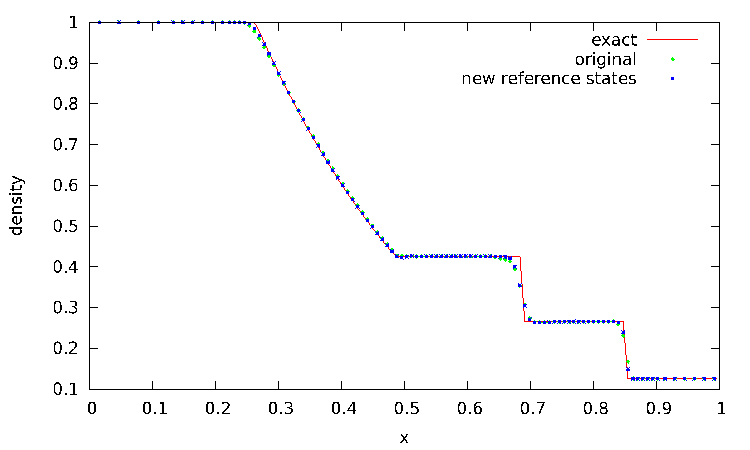
\includegraphics[scale=1.0]{plots/reference}
  \caption{ \label{Fig:sod} Solution to Sod's problem with the original
    reference state and the new reference state, as compared to the
    exact solution.  We note that the new reference state shows a
    slightly sharper shock and contact, but also has a dip at the tail
    of the rarefaction.}
\end{figure}

\clearpage

\end{document}

